\chapter{让整段曲线有地方走：安全走廊}
\begin{notebox}
\textbf{目标}\quad 沿 A* 路径构建整块安全的凸区域，并为后续轨迹分配走廊和连接点。\\
\textbf{先修}\quad 第 11、12 章；凸集、线段与半平面。
\end{notebox}

\section{先比较矩形与凸多边形}
\begin{lstlisting}[language=bash]
ros2 run motion2d corridor_demo tmp/ch13_corridor
/usr/bin/python3 scripts/plot_ch13_corridor.py
\end{lstlisting}
本章先使用给定栅格隔离算法，输入是已经膨胀的配置空间和原始 A* 邻格折线。
实验路线从隔墙左下方绕到上端，再回到右下方。先得到一串相互交叠的局部矩形，
再尝试合并成较少的凸多边形；每次合并都重新检查整个区域。

\section{一个凸区域的两种表示}
顶点表示适合画图；半空间表示适合写约束。对逆时针多边形，边从 $a_i$ 指向 $a_{i+1}$，
内部在边的左侧。令 $e_i=a_{i+1}-a_i$，单位外法向为
\begin{equation}
n_i=\frac{(e_{iy},-e_{ix})^T}{\|e_i\|},\qquad
b_i=n_i^Ta_i,\qquad \mathcal C=\{p\mid A p\leq b\}.
\end{equation}
$A$ 的第 $i$ 行是 $n_i^T$，各行法向长度均为 1；故 $n_i^Tp-b_i$ 是到该边直线的带符号距离，单位 m。
它非正表示点在此半平面中。一个点必须满足所有行，才属于整个区域。
\lstinputlisting[language=C++,linerange={corridor_halfspace_begin-corridor_halfspace_end},
  includerangemarker=false]{../ros2_ws/src/motion2d/src/planning/corridor.cpp}

\begin{notebox}
\textbf{已经在配置空间内}\quad 走廊容纳的是机器人圆心，输入格子的半径和安全裕量已在第十一章处理。
这里不再次缩小一个物理半径。只有半空间约束正确且整个区域安全，才能使用后面的凸性论证。
\end{notebox}
公开接口为 makeRegion、regionIsFree 和 buildCorridor；结果同时保留顶点与半空间。
凸多边形须严格凸、逆时针且非退化。练习 ch13-1 从一条边写出对应的单位外法向和偏移。

\clearpage
\section{从局部矩形开始}
对每一段原始邻格路径，取起终点所在格子的包围框。若点恰好在格线或格角上，种子包含两侧格子。
框内每格都自由才可开始扩张，然后轮流尝试向左、右、下、上增加一条完整栅格边。
任何新增格被阻塞，就不接受这次扩张。每侧还有局部扩展长度限制 $L$，对应最多
$\lfloor L/\rho\rfloor$ 格；演示设置 $L=0.6$ m。
\lstinputlisting[language=C++,linerange={corridor_rectangle_begin-corridor_rectangle_end},
  includerangemarker=false]{../ros2_ws/src/motion2d/src/planning/corridor.cpp}
输出边界向内缩 $10^{-6}\rho$，在浮点运算下保留与阻塞格的分离。
每条种子线段的两个端点仍须在矩形内，所有边界约定与完整区域检查一致。
如果当前最后一个矩形已经包含下一段的两个端点，就无需重复添加。
扩张顺序会影响形状；这不是最大面积矩形求解器，合并后的区域也不再受单个种子的扩展窗口限制。

\section{安全顶点不足以证明区域安全}
一个四边形的四个顶点、甚至四条边都可能自由，而小障碍被包在正中间。
因此 regionIsFree 遍历区域包围框内的\textbf{阻塞方格}，求它们与走廊多边形的闭集交集。
只要交集非空，就拒绝；擦角或沿边接触也算非空。

实现对多边形逐次施加方格的四个半平面约束。跨越某个边界 $n^Tp=b$ 的边段，
设两端残差为 $\alpha=n^Tp_0-b$、$\beta=n^Tp_1-b$，交点为
\begin{equation}
p_\ast=p_0+\frac{\alpha}{\alpha-\beta}(p_1-p_0).
\end{equation}
保留半平面内的顶点与必要交点，重复四次。碰撞检查保留退化的点和线，避免漏掉接触。
地图外部也被拒绝。检查针对整块区域，不需要靠稠密采样猜测内部是否安全。

\section{只有通过验证才合并}
把相邻矩形顶点放在一起求凸包，再调用同一个 regionIsFree。
通过则替换成凸包，否则保留两个已有区域。转弯内侧的障碍经常导致合并失败，这是应保留的约束。
浮点近共线顶点若不满足严格凸性，也放弃该次可选合并。
局部矩形刻意有扩展窗口，因此在更大自由空间中，合并后可以出现六边形等非矩形区域。

\clearpage
\section{交叠区域决定连接点}
设相邻两个走廊为 $\mathcal C_i,\mathcal C_{i+1}$，先求交集
\begin{equation}
\mathcal I_i=\mathcal C_i\cap\mathcal C_{i+1}.
\end{equation}
它也由凸半平面裁剪得到。这里要求\textbf{正面积}，只共用一条边或一个点不够。
数值阈值为 $10^{-10}\rho^2$；这个阈值只排除退化交叠，实际运动余量仍受地图与半径决定。
从交集多边形的顶点 $v_1,\ldots,v_K$ 取平均作为连接点：
\begin{equation}
q_i=\frac1K\sum_{k=1}^K v_k.
\end{equation}
这是一个容易计算的内部点，不是多边形的面积质心，也不保证最大净空。
起点和终点采用原始请求坐标，最终 $N$ 个走廊对应 $N+1$ 个路点。
第 $i$ 条新线段的两个端点都属于 $\mathcal C_i$，于是由凸性有
\begin{equation}
(1-s)q_i+s q_{i+1}\in\mathcal C_i,\qquad 0\leq s\leq1.
\end{equation}
这证明的是\textbf{分配后的直线段}整段包含在安全区域。
经过相同路点的五次曲线可能向外鼓出，不能直接复用这条证明；第十六章会检查整段 Bezier 凸包。

\section{失败时不返回半成品}
\begin{center}\small
\begin{tabular}{ll}\toprule
状态 & 含义 \\\midrule
empty\_path & 没有可用路径 \\
unsafe\_path & 原始折线含越界、穿障或接触 \\
blocked\_seed\_box & 线段安全，但整格种子框不可用 \\
no\_positive\_overlap & 相邻区域没有正面积交叠 \\
invalid\_extension & 扩展长度参数不合法 \\\bottomrule
\end{tabular}
\end{center}
失败结果的区域和路点均为空，调用方应保留明确失败状态。
尤其不要把贪心简化后的长对角线直接拿来扩张矩形：线段可以绕过方格，包围框却可能覆盖它。
保留原始 A* 邻格路径更适合本章构造方式；已有长线段可另行重新离散搜索。

验证覆盖单位法向、几何包含、点/线退化交叠、内部障碍、擦边/擦角、非矩形安全凸包、
转弯路线与不同栅格尺度。对每个最终区域验证整块无碰撞，并检查分配给它的两个端点。
这些是地图所表达的几何证书，仍依赖观测质量与定位质量。

\clearpage
\section{固定地图上的对照实验}
\begin{figure}[h]
\centering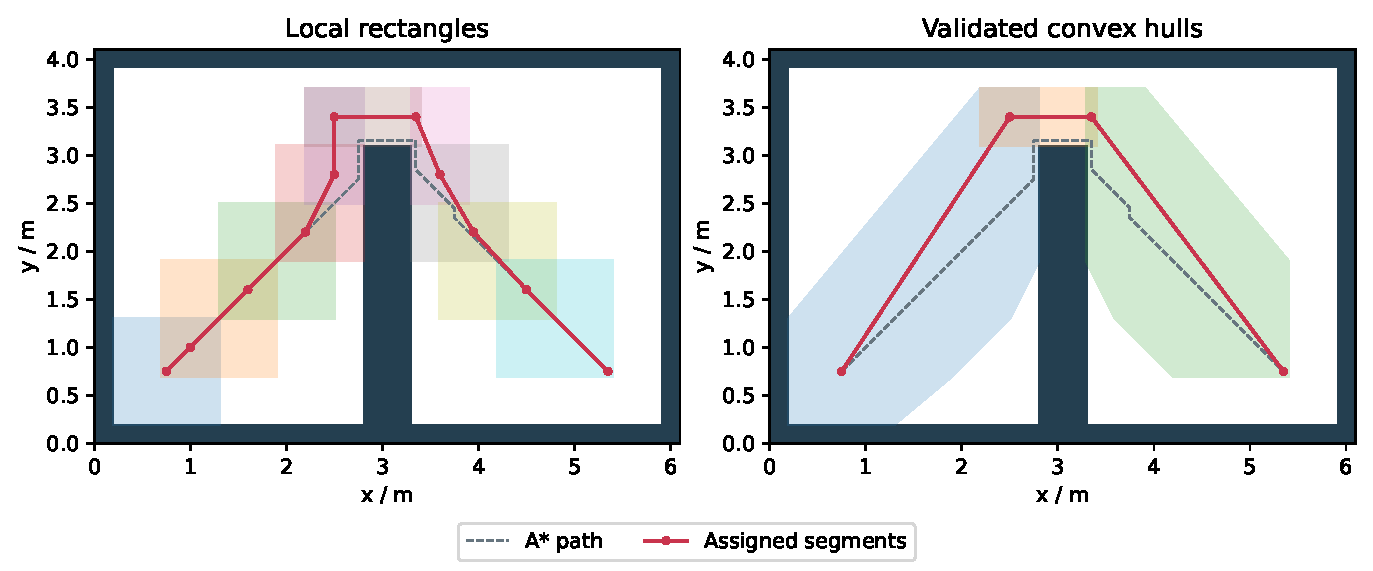
\includegraphics[width=\linewidth]{figures/ch13_corridor.pdf}
\caption{深色为已膨胀阻塞格，浅色为走廊，虚线为原始 A* 路径。
红色线段的两个端点均分配到同一个凸区域中。两图采用相同坐标比例。}
\end{figure}
\begin{center}\small
\pgfplotstabletypeset[col sep=comma,
columns={convex,regions,vertices,waypoints,min_overlap_area_m2},
columns/convex/.style={column name=凸包合并,string type,string replace*={0}{关},string replace*={1}{开}},
columns/regions/.style={column name=区域数},columns/vertices/.style={column name=总顶点数},
columns/waypoints/.style={column name=路点数},
columns/min_overlap_area_m2/.style={column name=最小交叠/$m^2$,fixed,precision=3},
every head row/.style={before row=\toprule,after row=\midrule},
every last row/.style={after row=\bottomrule}]{data/ch13_corridor.csv}
\end{center}
给定图为 $61\times41$ 格，分辨率 0.1 m，半径 0.15 m，额外裕量为零。
隔墙上端留出绕行空间，起终点分别为 $(0.75,0.75)$、$(5.35,0.75)$ m。
在完全相同的 A* 路径上，局部矩形为 10 个，安全凸包合并后为 3 个；总顶点数从 40 变成 19。
两种构造的最小交叠面积都约为 $0.06\,m^2$，所以连接点没有落在仅共边的退化位置。

区域变少会减少后续轨迹分段和约束的组织成本，但不代表最短路径、最小 jerk 或最大走廊体积。
本章没有给红线分配时间，也没有直接驱动机器人。

\begin{enumerate}
\item \textbf{理解：}画一个内部含障碍的凸四边形，说明只测顶点和边会遗漏什么。
\item \textbf{代码 ch13-1：}把 CCW 边转为单位半空间。底边 $(1,2)\to(4,2)$ 给出 $-y\leq-2$；
斜边 $(4,2)\to(7,6)$ 的外法向为 $(0.8,-0.6)$。
\item \textbf{实验：}改变局部扩展长度与合并开关，记录区域数、形状与最小交叠面积。
保持地图、半径和路径相同，解释变化原因。
\end{enumerate}
ROS 观测路径上的走廊显示将在下一功能接入。
